\documentclass[a4paper,12pt]{article}
\usepackage[utf8]{inputenc}
\usepackage{geometry}
\geometry{a4paper, margin=1in}
\usepackage{hyperref}
\usepackage{graphicx}
\usepackage{titlesec}
\usepackage{booktabs}
\usepackage{amsmath}

\titleformat{\section}{\normalfont\Large\bfseries}{\thesection}{1em}{}[\titlerule]

\begin{document}
\begin{center}
    \textbf{\Huge Theory Answers }\\
    \vspace{0.2 cm}
    \textbf{\Huge Juan José Lozano González}\\
    \vspace{0.2 cm}
    \textbf{\Huge First Lab PHY 192}\\
    \rule{\textwidth}{0.4pt}
\end{center}

\vspace{1cm}

\noindent \textbf{\LARGE Question 1.1}

\vspace{0.2cm}

Refraction is the process by which light bends as it goes from one medium to another. This bending is caused by the change in speed of light as it goes from one medium to another, and due to the fact that light always takes the shortest path (in time) between 2 points.

\vspace{0.2cm}

\noindent \textbf{\LARGE Question 1.2}

\vspace{0.2cm}

The index of refraction is unitless as it is defined as the ratio between the speed of light in a vacuum, and the speed of light in the given medium. As such it is impossible it is impossible to have a index of refraction of less than one as that implies light going faster than the speed of light in a vacuum which is physically impossible.

\vspace{0.2cm}

\noindent \textbf{\LARGE Question 1.3}

\vspace{0.2cm}

The effect shown in the photo is called total internal reflection, which makes the medium a - medium b barrier act like a mirror, however if the angle of incidence is of 0 this effect cannot occur, as such whether one can look out of the water or not depends on the angle of incidence.

\vspace{0.2cm}

\noindent \textbf{\LARGE Question 1.4}

\vspace{0.2cm}

As the index of refraction is inversely proportional to the square of the wavelength of light ($n \propto \frac{1}{\lambda^2}$), blue should have a larger index of refraction than blue because red has a smaller bandwidth. For reference the normally recognized wavelength for blue light is approximately 450-495 nm, and for red light, it is approximately 620-750 nm.

\vspace{0.2cm}

\noindent \textbf{\LARGE Question 1.5}

\vspace{0.2cm}

For refraction to occur the angle of incidence of the light must be non zero, the angle of incidence being defined as the angle formed by the ray of light and the normal vector to the medium-medium interface, with this logic in mind it is to be expected that rays of light h and f are going to be refracted, while ray of light g is not expected to refract.

\vspace{0.2cm}

\noindent \textbf{\LARGE Question 1.6}

\vspace{0.2cm}

I see the ray of light enter at 234° and exit at 312°, however my eyes are bad so I will give it twice the minimum unit of division of the apparatus of measurement which is 0.5°.

\vspace{0.1cm}

As such I believe the angle $\phi$ is 312° - 234° = 78° $\pm$ 1°.

\vspace{3cm}

\noindent \textbf{\LARGE Question 1.7.a}

\vspace{0.2cm}

We have that:

\begin{equation}
    \sin(\theta_1) = n \sin(\theta_2)
\end{equation}

\vspace{0.2cm}

\noindent \textbf{\LARGE Question 1.7.b}

\vspace{0.2cm}

The curve described by the relation between $\theta_1$ and $\theta_2$ is that of the sinh.

\vspace{0.4cm}

\noindent \textbf{\LARGE Question 1.7.c}

\vspace{0.2cm}

With the requested change of variables we have that:

\begin{equation}
    Y = n X
\end{equation}

With given plot.

\begin{figure}[h]
    \centering
    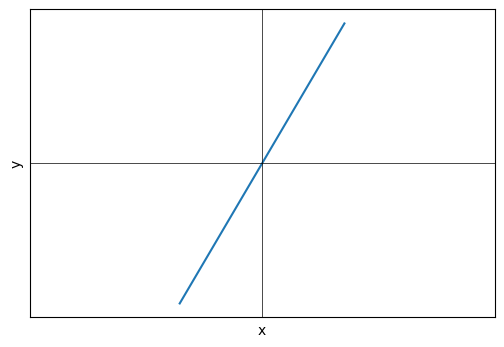
\includegraphics[width=0.5\textwidth]{First Lab Theory first image.png}
    \caption{Here is the graph of the function $Y = nX$} 

\vspace{0.5cm}

\noindent{From this equation it also obvious that the slope of this function is n.}


\end{figure}

\end{document}
